\section{Introduction}

Resolution is where trust concentrates in prediction markets. A market can make its pricing, accounting, and settlement rules executable. It must still connect those rules to something that happened outside the contract. The question is not whether trust is required, but whether it is visible.

The companion paper on trust-explicit resolution \cite{trustexplicit2026} proposes that every market carry an executable resolution constitution: declared sources, judgment steps, decision rules, dispute paths, and funding. That fixes what the resolver is supposed to do. The next question is simpler: how does anyone know the resolver did it?

A proposer can fabricate a plausible trace, submit a bonded result, and bet that nobody will check. A signature identifies who endorsed that claim. A hash prevents later editing. Neither alone establishes that the declared program ran. This is the execution integrity gap. It is distinct from the truth problem. An authentic runner can faithfully process a false source report. A fabricated execution can accidentally produce the right answer. Both distinctions matter when money settles on the result.

This paper closes parts of that gap with a progressive verification stack:
\begin{enumerate}
\item \textbf{Blueprint commitment} fixes the decision program and its fallback rules before trading.
\item \textbf{Trace commitment and publication} fix a complete, inspectable account of the claimed run and make individual disputes compact.
\item \textbf{Execution assurance} binds that account to a runner identity, an attested execution environment, or a committee with an explicit fault model.
\item \textbf{Economic fallback} funds the checking and adjudication that remain necessary outside those guarantees.
\end{enumerate}

The stack also needs a common execution request. It binds the market, blueprint, source snapshot, permitted attempts, and acceptance policy. Otherwise a perfectly attested runner can repeatedly execute a stochastic workflow and submit whichever result it likes. Verifying an invocation is not enough. The protocol must verify that this was an authorized invocation and account for attempts that disappeared.

\begin{figure}[t]
\centering
\resizebox{0.98\linewidth}{!}{\begin{tikzpicture}[
  x=1cm, y=1cm,
  every node/.style={font=\sffamily},
  >={Stealth[length=2.2mm]},
  % ── Main stack layers ────────────────────────────────────────────
  layer/.style={
    text width=7cm, minimum height=1.2cm,
    align=left, inner sep=7pt,
    rounded corners=4pt, line width=0.65pt,
    font=\sffamily\fontsize{9.5pt}{11.5pt}\selectfont,
  },
  qcore/.style={layer, draw=blue!50!black, fill=blue!6},
  qecon/.style={layer, draw=orange!35!black, fill=orange!5},
  % ── Side annotations ────────────────────────────────────────────
  annot/.style={
    text width=4.4cm, minimum height=1.2cm,
    align=left, inner sep=7pt,
    rounded corners=4pt, line width=0.55pt,
    font=\sffamily\fontsize{8.5pt}{10.5pt}\selectfont,
  },
  qadds/.style={annot, draw=teal!50!black, fill=teal!4},
  qout/.style={annot, draw=black!38, fill=black!3},
  % ── Misc ─────────────────────────────────────────────────────────
  note/.style={
    font=\sffamily\fontsize{7.8pt}{9.5pt}\selectfont,
    text=black!48, align=left, text width=13cm,
  },
  ftitle/.style={
    font=\sffamily\bfseries\fontsize{13pt}{14.5pt}\selectfont,
    text=black!78,
  },
  flow/.style={->, line width=0.85pt, draw=black!46},
  conn/.style={->, line width=0.6pt, draw=black!28, dashed},
]

% ── Title ──────────────────────────────────────────────────────────
\node[anchor=west, ftitle] at (0, 0.5) {Progressive verification stack};

% ── Stack layers ───────────────────────────────────────────────────
\node[qcore] (L1) at (3.75, -1.0) {%
  \textbf{1.\enspace Blueprint commitment}\\[1pt]
  {\footnotesize Market commits to a declared decision program.}};

\node[qcore] (L2) at (3.75, -2.85) {%
  \textbf{2.\enspace Merkle trace commitment}\\[1pt]
  {\footnotesize Proposal pins the claimed run, node-by-node, at proposal time.}};

\node[qcore] (L3) at (3.75, -4.7) {%
  \textbf{3.\enspace Execution assurance}\\[1pt]
  {\footnotesize Signatures bind identity; attestation adds a measured environment.}};

\node[qecon] (L4) at (3.75, -6.55) {%
  \textbf{4.\enspace Economic fallback}\\[1pt]
  {\footnotesize Bonds, challenges, and adjudication handle everything outside the attestation boundary.}};

% ── Vertical flow ─────────────────────────────────────────────────
\draw[flow] (L1) -- (L2);
\draw[flow] (L2) -- (L3);
\draw[flow] (L3) -- (L4);

% ── Side: what each layer adds ────────────────────────────────────
\node[qadds] (adds) at (10.7, -2.85) {%
  \textbf{What each layer adds}\\[2pt]
  {\footnotesize
  Declared logic\\
  Pinned trace contents\\
  Bound execution identity\\
  Challengeable residual risk}};

% ── Side: still outside ───────────────────────────────────────────
\node[qout] (outside) at (10.7, -6.25) {%
  \textbf{Still outside the boundary}\\[2pt]
  {\footnotesize
  External truth and source correctness\\
  LLM or human judgment quality\\
  Host availability and liveness\\
  Registrar and hardware-vendor trust}};

% ── Connecting arrows (split targets to avoid overlap) ────────────
\draw[conn] (L2.east) -- (adds.172);
\draw[conn] (L3.east) -- (adds.188);
\draw[conn] (L4.east) -- (outside.west);

% ── Bottom note ────────────────────────────────────────────────────
\node[note, anchor=north west] at (0, -8.0) {%
  Blueprints define the rules. Traces pin the claimed run.
  Execution assurance narrows fabrication risk.
  Economic fallback handles the rest.};

\end{tikzpicture}
}
\caption{Progressive verification. The execution request, publication gate, and challenge policy bind the layers into one resolution procedure.}
\label{fig:stack}
\end{figure}

\subsection{Contributions}

Markets should progressively improve the evidence that their committed decision program actually ran. This paper gives that thesis a concrete protocol and a set of testable claims.

First, the two-axis trust model separates \emph{what kind of judgment determines the outcome} from \emph{what supports the execution claim}. A deterministic source rule with anonymous execution and an LLM judgment with attested execution have different risks. A single trust score obscures that distinction.

Second, a bounded reference protocol specifies canonical bytes, a count-bound Merkle tree, complete trace semantics, authenticated source objects, and a publication state machine. We prove what an accepted trace establishes and give explicit omission and forgery counterexamples for weaker checks. The protocol uses a full-trace hash as its baseline: Merkle structure adds compact authenticated openings, not a new guarantee that the original account was honest.

Third, we separate each runner's evidence receipt from the shared result on which a committee agrees. We derive quorum safety, liveness, trust-domain constraints, and attempt-selection bounds. These identify exactly when replication strengthens assurance and when it merely repeats the same dependency.

Finally, executable adversarial tests, independent commitment implementations, exact committee enumeration, seeded selection experiments, and compiled AVM measurements exercise the repaired design. The research artifacts are independent of question.market's current implementation. They establish properties of the declared research protocol, with hardware deployment and field behavior left as separately specified experiments.

\subsection{Related work and current direction}

\textbf{Declared resolution and disputes.} Optimistic oracles and bonded-answer systems make a claim contestable. The companion paper supplies the dispute economics and declared workflow for this design \cite{trustexplicit2026}. Here the object being contested is the execution of that workflow. We do not assume that the presence of a bond guarantees an attentive verifier.

\textbf{Authenticated computation and fraud proofs.} Town Crier supplies TEE-backed authenticated data feeds; Ekiden separates confidential execution from consensus \cite{towncrier2016,ekiden2019}. Arbitrum's optimistic computation makes incorrect off-chain execution claims subject to narrow on-chain disputes \cite{arbitrum2018}. Our local trace challenges use this established separation between a commitment and a proof of an invalid transition. A Merkle inclusion proof authenticates the disputed record; a semantic check establishes the fault.

\textbf{Replicated confidential execution.} Chainlink Confidential Compute already specifies replicated enclaves, result comparison, and threshold-generated deterministic randomness; it also describes a ZK execution tier \cite{chainlinkcc}. The contribution here is not the invention of replicated TEEs. It is a market-resolution protocol that binds requests, attempts, complete evidence, quorum composition, and disputes to the constitution chosen before trading.

\textbf{Attestation and release transparency.} The RATS architecture distinguishes the attester, verifier, and relying party \cite{rats2023}. This maps naturally to the enclave, registrar, and market contract. Apple's Private Cloud Compute requires attested measurements to appear in a public release-transparency log \cite{pcc2026}. That is a useful precedent for making the source-to-measurement mapping inspectable instead of treating a measurement as an unexplained allowlist entry.

\textbf{Source and model provenance.} DECO and TLSNotary address evidence of data obtained from authenticated TLS sources \cite{deco2020,tlsnotary}. AEX, a March 2026 preprint, studies signed provenance across LLM API intermediaries and explicitly distinguishes endpoint accountability from proof of model inference \cite{aex2026}. An August 2026 technical note combines action evidence with RATS-style attestation in an emulated TPM experiment \cite{aep2026}. These are relevant developing directions, not demonstrations that a remotely hosted model executed inside this paper's runner enclave.

\textbf{Proofs and persistent state.} zkLLM demonstrates that proving substantial model computation is a concrete research program, making a blanket claim that ZK execution is infeasible untenable \cite{zkllm2024}. Rollback-resistant storage work likewise shows why protected execution memory does not by itself supply persistent one-shot state \cite{teerex2026}. This design therefore places request authorization and attempt consumption in an authoritative ledger, and treats proof-carrying deterministic subgraphs as a promising extension.

\section{The Two-Axis Trust Model}
\label{sec:twoaxis}

The resolution class describes the decision program:
\begin{itemize}
\item \textbf{Source-based}: declared computations over external or on-chain records, without model-mediated or human judgment.
\item \textbf{Agent-assisted}: at least one model-mediated judgment. A fixed local model with fixed decoding can be deterministic; determinism does not remove its judgment role.
\item \textbf{Human-judged}: at least one human decision. Recorded testimony can be replayed as an input even when the underlying judgment cannot be recomputed.
\end{itemize}
When a workflow mixes classes, its displayed primary label gives human judgment precedence over model judgment over source processing, while retaining the full list of dependencies. This is a display convention, not an ordering of safety.

Execution assurance describes the support for a particular submitted claim:
\begin{itemize}
\item \textbf{Unauthenticated}: a commitment fixes the account, without an approved execution identity.
\item \textbf{Signed runner}: an authorized key endorses the request-bound receipt.
\item \textbf{TEE-attested}: an appraised hardware attestation binds that key to an approved measured environment under a declared registration policy.
\item \textbf{Threshold TEE-attested}: an eligible committee supplies a certificate satisfying explicit signer and trust-domain rules.
\end{itemize}
The four named modes give twelve descriptive combinations with the three resolution classes. They are not a theorem that risks are statistically independent, nor a universal ladder on which every larger committee is safer. Replayability, input authentication, selection policy, availability, and shared trust dependencies remain visible descriptors.

\begin{figure}[t]
\centering
\resizebox{0.98\linewidth}{!}{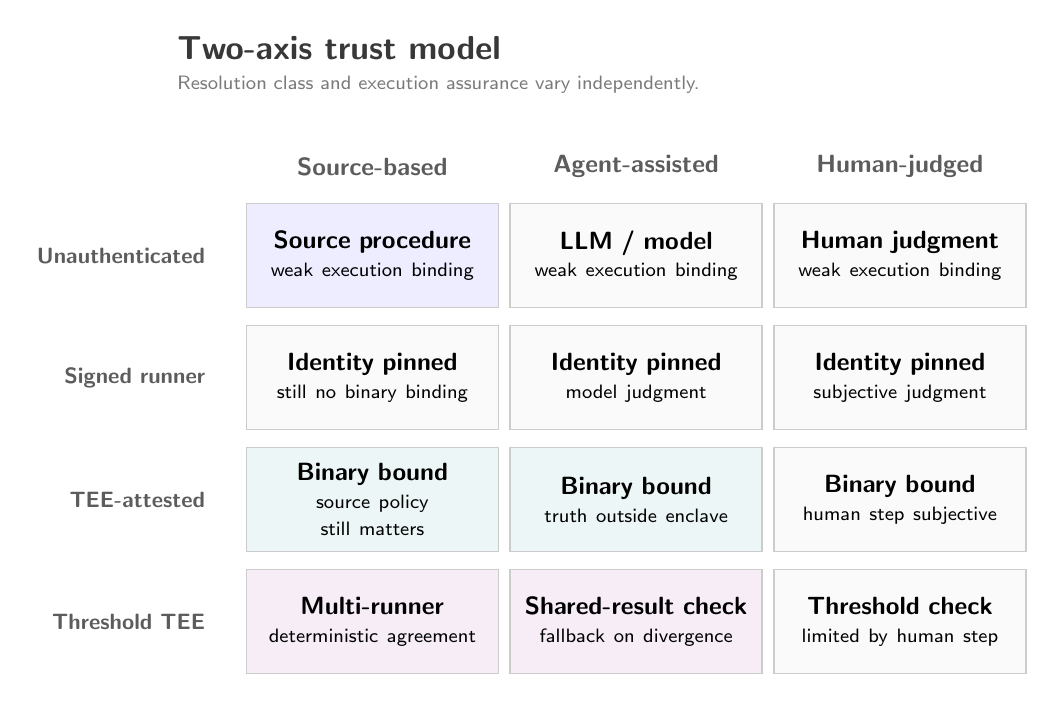
\begin{tikzpicture}[
  x=1cm, y=1cm,
  every node/.style={font=\sffamily},
  % ── Typography ───────────────────────────────────────────────────
  ftitle/.style={
    font=\sffamily\bfseries\fontsize{12.8pt}{13.8pt}\selectfont,
    text=black!78,
  },
  axislbl/.style={
    font=\sffamily\bfseries\fontsize{8.9pt}{9.9pt}\selectfont,
    text=black!68,
  },
  rowhead/.style={
    font=\sffamily\bfseries\fontsize{8.4pt}{9.4pt}\selectfont,
    text=black!64, align=right,
  },
  colhead/.style={
    font=\sffamily\bfseries\fontsize{8.6pt}{9.6pt}\selectfont,
    text=black!64, align=center,
  },
  small/.style={
    font=\sffamily\fontsize{7.3pt}{8.2pt}\selectfont,
    text=black!52, align=center,
  },
  % ── Grid cells ───────────────────────────────────────────────────
  cell/.style={
    draw=black!20, line width=0.55pt,
    minimum width=3.15cm, minimum height=1.32cm,
    text width=2.85cm,
    align=center, inner sep=5pt,
    font=\sffamily\fontsize{8.7pt}{10pt}\selectfont,
  },
  hi1/.style={cell, fill=blue!7},
  hi2/.style={cell, fill=teal!7},
  hi3/.style={cell, fill=violet!7},
  base/.style={cell, fill=black!2},
]

% ── Title ──────────────────────────────────────────────────────────
\node[anchor=west, ftitle] at (-0.05, 0.78) {Two-axis trust model};
\node[anchor=west, small] at (-0.05, 0.32) {Resolution class and execution assurance vary independently.};

% ── Column headers ─────────────────────────────────────────────────
\node[colhead] at (2.55, -0.72) {Source-based};
\node[colhead] at (5.90, -0.72) {Agent-assisted};
\node[colhead] at (9.25, -0.72) {Human-judged};

% ── Row headers ────────────────────────────────────────────────────
\node[rowhead, anchor=east] at (0.55, -1.85)  {Unauthenticated};
\node[rowhead, anchor=east] at (0.55, -3.40) {Signed runner};
\node[rowhead, anchor=east] at (0.55, -4.95)  {TEE-attested};
\node[rowhead, anchor=east] at (0.55, -6.50) {Threshold TEE};

% ── Row 1: Unauthenticated ────────────────────────────────────────
\node[hi1]  at (2.55, -1.85)  {\textbf{Source procedure}\\{\scriptsize weak execution binding}};
\node[base] at (5.90, -1.85)  {\textbf{LLM / model}\\{\scriptsize weak execution binding}};
\node[base] at (9.25, -1.85)  {\textbf{Human judgment}\\{\scriptsize weak execution binding}};

% ── Row 2: Signed runner ──────────────────────────────────────────
\node[base] at (2.55, -3.40) {\textbf{Identity pinned}\\{\scriptsize still no binary binding}};
\node[base] at (5.90, -3.40) {\textbf{Identity pinned}\\{\scriptsize model judgment}};
\node[base] at (9.25, -3.40) {\textbf{Identity pinned}\\{\scriptsize subjective judgment}};

% ── Row 3: TEE-attested ───────────────────────────────────────────
\node[hi2]  at (2.55, -4.95)  {\textbf{Binary bound}\\{\scriptsize source policy still matters}};
\node[hi2]  at (5.90, -4.95)  {\textbf{Binary bound}\\{\scriptsize truth outside enclave}};
\node[base] at (9.25, -4.95)  {\textbf{Binary bound}\\{\scriptsize human step subjective}};

% ── Row 4: Threshold TEE ──────────────────────────────────────────
\node[hi3]  at (2.55, -6.50) {\textbf{Multi-runner}\\{\scriptsize deterministic agreement}};
\node[hi3]  at (5.90, -6.50) {\textbf{Shared-result check}\\{\scriptsize fallback on divergence}};
\node[base] at (9.25, -6.50) {\textbf{Threshold check}\\{\scriptsize limited by human step}};

\end{tikzpicture}
}
\caption{The two axes describe different facts. Replayability additionally depends on the input snapshot and runtime; a model-based decision can be deterministic, and an unsigned live source can be impossible to replay.}
\label{fig:twoaxis}
\end{figure}

For market $M$, blueprint $G$, proposal $P$, and ledger time $t$, write
\[
\mathcal T(M,P,t)=\bigl(\kappa(G),\epsilon_{\rm req}(M),
\epsilon_{\rm run}(P,t),\rho,\sigma,\eta,\mathcal D\bigr).
\]
Here $\rho$ records replayability and source authentication, $\sigma$ the attempt-selection rule, $\eta$ publication and fallback policy, and $\mathcal D$ the dependency graph of operators, registrars, vendors, builds, and sources. The market declares a required mode at creation. The realized mode is checked against the receipt and current registry; an expired key or unavailable quorum cannot silently downgrade it.

The profile is descriptive, not prescriptive. It tells participants what they are relying on. A participant can prefer a transparent deterministic source computation to an attested subjective judgment without pretending that the latter's execution evidence is worthless. Trust becomes visible enough to price.

\section{Security Model and Protocol Objects}
\label{sec:model}

The adversary can operate the proposer and host, choose when to send messages, withhold evidence, restart processes, control allowed faulty committee members, and corrupt declared trust domains. It can supply arbitrary traces and unauthenticated network bytes. It cannot forge an honest source or runner signature, find hash collisions, or change finalized ledger state under the corresponding cryptographic and ledger assumptions. TEE claims additionally assume the declared hardware and measured-code boundaries hold. These assumptions are separate: a broken registrar can defeat an otherwise intact enclave.

The adversary's objectives are to finalize an outcome inconsistent with the declared computation, conceal a required input or step, substitute an unauthorized execution, select a favorable stochastic result, or block resolution. Source falsity and poor judgment are distinct objectives handled by source policy and adjudication. A valid execution proof is compatible with a wrong real-world answer.

\subsection{One request, distinct evidence receipts}

Before execution, an authoritative request fixes the chain and market identity, blueprint and semantics version, input-snapshot commitment, permitted attempt policy, authorized runners, timing, and publication rule. Its identifier $q$ is a domain-separated digest of the canonical request. The snapshot fixes the exact source objects or the rule by which independently authenticated objects become fixed; a URL and a loose time window alone do not identify common input bytes.

Runner $j$ produces its own receipt $E_j$, binding $q$, its run identity and measurement, the complete trace root and count, and the shared result digest $d$. The common result contains $q$ and the declared terminal output. It excludes run-specific timestamps, trace locations, keys, and measurements. In a committee, every signature binds both $d$ and $E_j$:
\[
\operatorname{Sig}_{K_j}\!\left(H(\mathrm{domain},d,E_j)\right).
\]
The concrete encoding is versioned; this notation denotes an unambiguous typed object, not raw concatenation of variable-length fields. An authorized receipt may have a different root from another receipt while endorsing the same result. That difference is expected, not evidence of dishonesty.

Agreement is meaningful only over the same $q$. For deterministic computation, identical authenticated inputs and semantics imply identical terminal results. For a stochastic or human step, the constitution must define fixed aggregation or a fallback on divergence. Deterministic descendants are compared conditional on equal parent inputs. Two honest computations fed different judgments need not agree merely because their later nodes are deterministic.

\subsection{Two different claims}

A complete trace plus successful replay establishes that the declared result is consistent with the declared computation over the recorded inputs. It does not establish the historical fact that the original proposer performed that work. An execution receipt can add provenance under its assurance assumptions. Neither fact establishes the truth of an external report.

Keeping these claims separate makes verification stronger. The protocol can reject a fabricated, inconsistent trace without asking which machine produced it. It can accept a consistent computation while exposing the precise source or judgment on which its conclusion rests. And it can demand stronger provenance when a market's constitution makes actual invocation, model identity, or exclusive key custody material.
